\section{Derivatore}

\begin{wrapfigure}[11]{r}[0pt]{65mm}
	\caption{Circuito derivatore}
	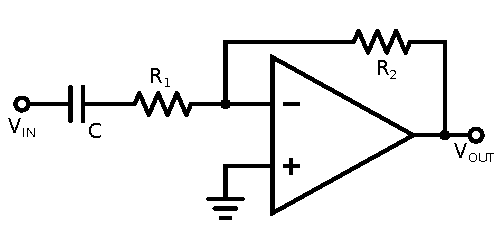
\includegraphics[width=65mm]{ccder.pdf}
	\label{fig:ccder}
\end{wrapfigure}

In quest'ultima parte dell'esperienza analizzeremo il circuito derivatore, il cui schema è riportato in Fig. \ref{fig:ccder}.
Anche in questo caso è banale ricavare l'equazione che lega $V_{out}$ a $V_{in}$: $C\frac{dV_{in}}{dt}=-\frac{V_{out}}{R_2}\Rightarrow V_{out}=-R_2C\frac{dV_{in}}{dt}$.

I valori di resistenze e capacità utilizzati sono $R_2=(9.95 \pm 0.01)$ \si{\kilo\ohm}, $R_1=(1007.9 \pm 0.2)$ \si{\ohm} e $C=(0.097 \pm 0.002)$ \si{\micro\farad}.

Come già fatto per il circuito integratore dobbiamo calcolare la frequenza di taglio prima di poter decidere la frequenza alla quale effettuare le misure.
Risulta immediato dalle considerazioni fatte nella precedente sezione ricavare $f=\frac{1}{2 \pi R^* C}$ con $R^*=R_2+R_1$.
Il valore numerico risulta essere $f \simeq \SI{144}{\hertz}$.
In questo caso è evidente che il segnale sarà smorzato per frequenze inferiori a quella di taglio. Abbiamo effettuato il campionamento alla frequenza di $\SI{100}{\hertz}$, abbastanza vicino alla frequenza di taglio da non avere smorzamenti evidenti.

I risultati sono riportati nel seguente grafico.

\begin{figure}[h]
	\centering
			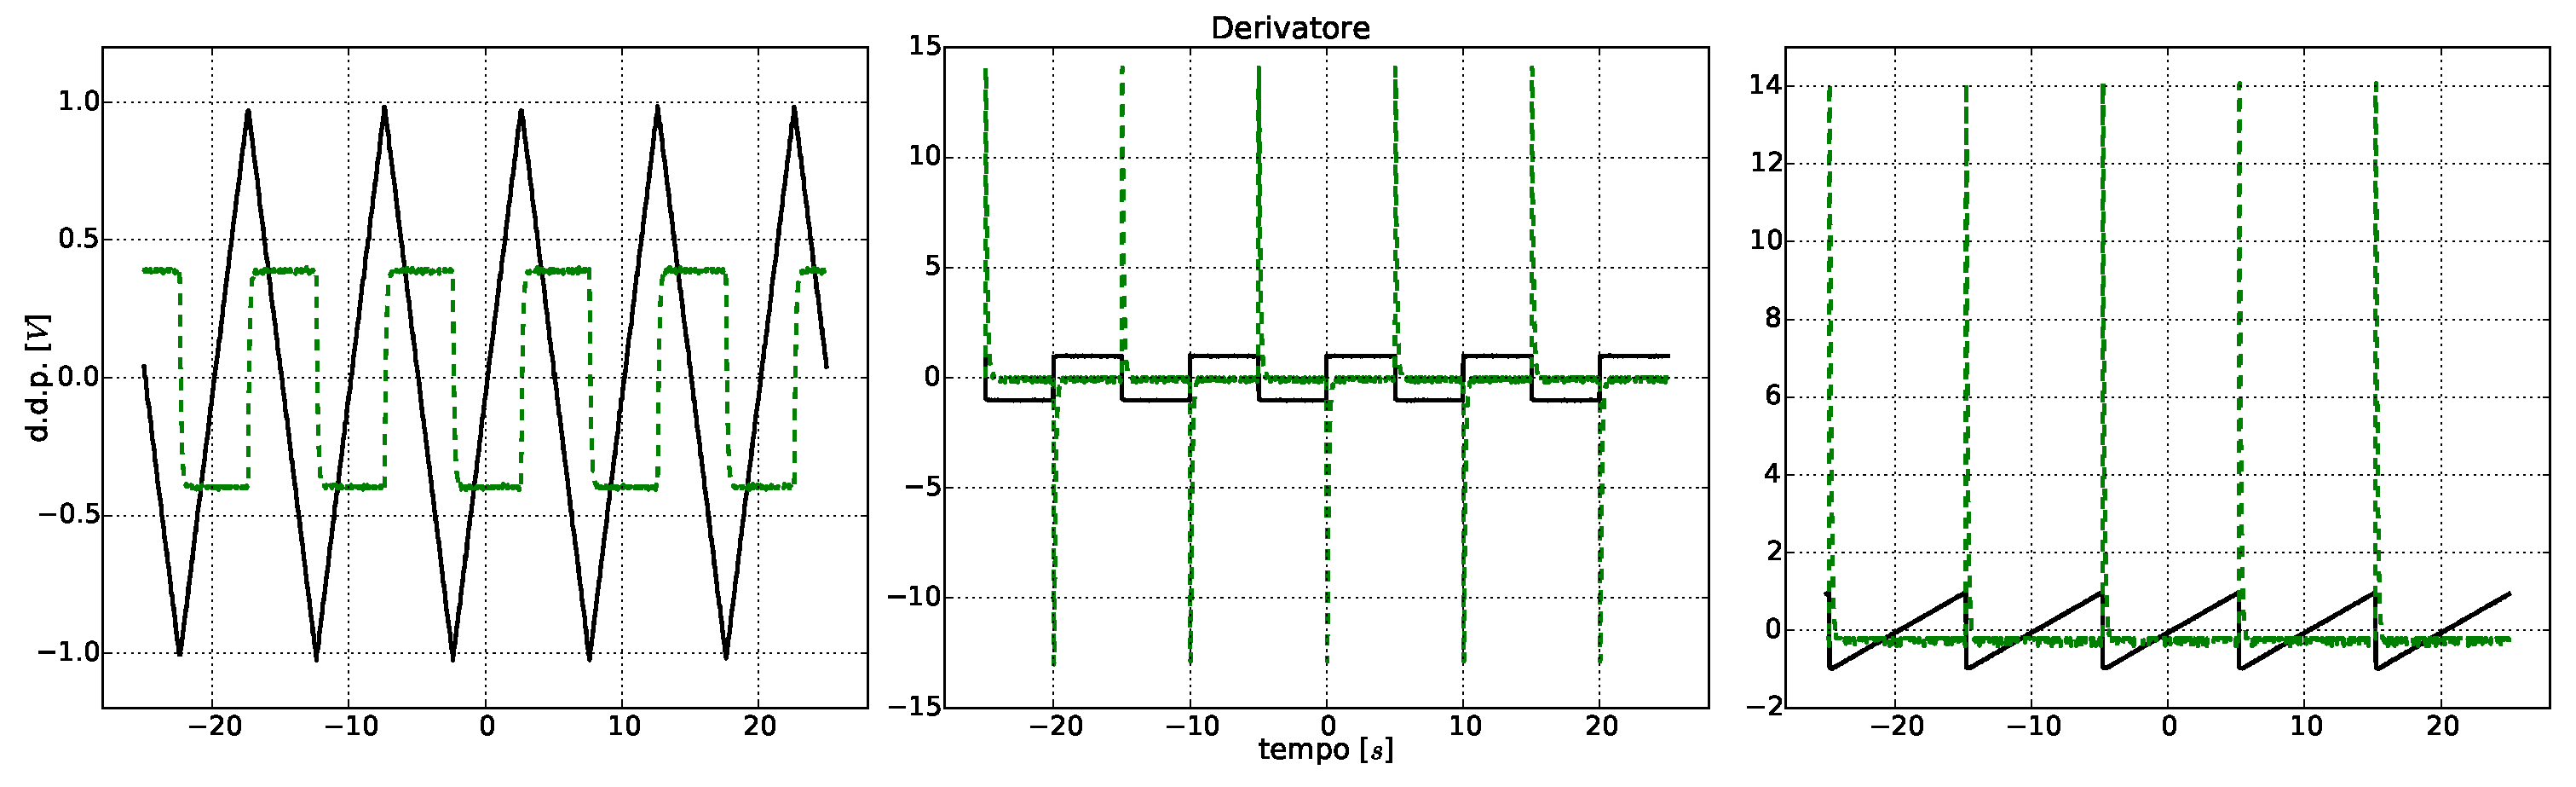
\includegraphics[width=.9\textwidth]{der_serie_10.pdf}
			\caption{Come vediamo graficamente in questo caso non è presente alcun offset in quanto il condensatore taglia i segnali continui in entrata. }
			\label{fig:der}
\end{figure}

Abbiamo provato ad aumentare la frequenza e abbiamo notato che il guadagno si stabilizzava su un valore di circa -10.
Questo risultato è coerente con la teoria, in quanto ad alte frequenze l'impedenza del condensatore diventa trascurabile e dunque il circuito diventa simile all'amplificatore invertente studiato nella prima sezione, con la differenza che esso amplifica la derivata del segnale.